\subsection{Debugger}\label{debugger}
The validation of the code generator lead to another validation-issue.
If a test program is not behaving as expected, is there a bug in the test program or in the compiler?

In other words:

\textit{How to validate the test programs?}

The answer to this is an embedded debugger in the target executable.

\fbox{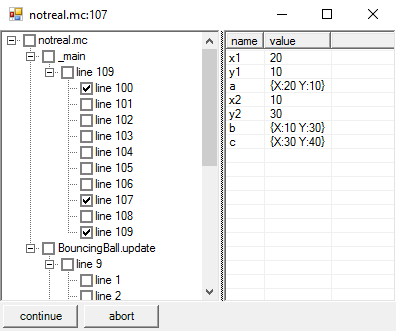
\includegraphics[width=\columnwidth-7pt]{debugger}}

The program will then trigger a breakpoint on the first instruction and launch the debugger GUI.
From the GUI, more breakpoints can be set with the check-boxes.
When the user presses `continue' or `abort', the GUI will close and appear again on the next breakpoint.

The left pane shows a four level deep tree which sorts the program on file name, function name, rule and line.

The right pane shows a table with the name and value of the local identifiers defined up to the current breakpoint.

\subsubsection{Output program changes}
When compiling with the debug flag set, some additions are made to target program.

\paragraph{Local identifier table}
After each instruction that defines named local identifiers, a new instruction is generated.

\begin{CS}
    var foo = 42;
    _dbug_symbol_table["foo"] = foo;
\end{CS}

After each assignment to a named local identifier, the named identifier and the value are recorded in a key-value collection. 
This key-value collection will be passed to the debugger when a breakpoint is hit.
A new key-value collection is defined at the start of each rule.

\paragraph{Break points}
When compiling with the debug-flag set, function closures will have a group of static boolean arrays.
One array for each rule in the function.

\begin{CS}[escapeinside=\#\#]
    class #\textit{<function name>}#{
        #\textit{<arguments>}#
        static bool[] _dbug_breakpoints_0;
        static bool[] _dbug_breakpoints_1;
        #\textit{<return value>}# _run(#\textit{<last argument>}#){
            #\textit{<body>}#
        }
    }
\end{CS}

The breakpoints are generated at each line of source code in the rule.
This is different than breaking at every instruction, as normalization often splits single lines into multiple instructions.

\begin{CS}
    ...
    if(_dbug_Breakpoints_1[6]){
        _dbug.breakpoint("filename.mc", 12, 
                         _dbug_symbol_table);
    }
    ...
\end{CS}

\subsubsection{Debug struct}
The breakpoint function is defined as a public static member of the debug struct.

The debugger is defined in a separate file, \verb|_dbug.cs|, which is imported by the target executable.
This is done to keep the program-specific code out of \verb|_dbug.cs|.

\verb|_dbug.cs| contains the struct \verb|_dbug|.
This struct contains only the following public static items.

\begin{enumerate}
    \item the program tree
    \item the breakpoint tree
    \item the breakpoint function
\end{enumerate}

The program builds up the program tree and the breakpoint tree in the main function, before the first user-written line starts.
The trees are both four-levels deep and sorted on filename, function name, rule and line number.
The breakpoint function is called when the program hits a break-point.

This was chosen because breakpoint checks happen every few instructions, so they have a huge effect on debug performance.
Straight arrays with booleans are very fast to index since it only costs one bounds-check, one addition and one dereference.
The dereference can even be done speculatively, due to branch prediction~\cite{branchprediction}.

\paragraph{The tree representation} of the program is four levels deep.
The first level represents the file, the second level represents the function, the third level represents the rule and the fourth level represents the premise.
This tree representation is initialized in the main function, before the user code begins.

\paragraph{The breakpoint table} 
Each closure has its group of breakpoints.
To easily index all the breakpoint arrays from one central point, the \verb|_dbug| struct has a breakpoint table.
The breakpoint table is a static four-dimensional array (\verb|bool[][][][]|) that points to the static breakpoint arrays in the closures.
This way, the arrays are quick to index from the closure, while being available in a tree-like from for the debugger.

\paragraph{The breakpoint function}
The \verb|_dbug| struct contains a static method \verb|breakpoint| that will pause the execution of the program and present the GUI.
When the user presses `continue' or `abort', the GUI will close and the \verb|breakpoint| method will return control back to the program.

The first two arguments to \verb|_dbug.breakpoint| are the filename and the line number to uniquely identify the call site.
The third argument is the symbol table that has been accumulated so far.

\subsubsection{Evolution}
The debugger has changed little, since it is a relatively simple construct.
The only significant changes were the decision to go from a single boolean array per closure to a boolean array per rule.
The book-keeping involved in having the boolean arrays packed was inelegant, because there was now a dependency between the rules: the latter breakpoint number depends on the breakpoints in the former rule.

